\documentclass[pdflatex,sn-basic]{sn-jnl}

% ---- packages ---------------------------------------------------------------
%  sn-jnl.cls already provides hyperref, natbib, url and the caption setup;
%  do not load those again or you will get an option clash.
\usepackage{graphicx}
\graphicspath{{assets/}}% figures live in assets/figures/; includes stay figures/...
\usepackage{amsmath,amssymb,amsfonts,bm}
\usepackage{booktabs}
\usepackage{array}
\usepackage{tabularx}
\usepackage{ragged2e}
\usepackage{xcolor}% revision marking; remove with the \color{red} blocks
% \snew{...}: student's merged-in changes from main-checking, bold green.
% Remove these \snew wrappers (and this line) once the merge review is done.
\definecolor{studentgreen}{rgb}{0.0,0.5,0.0}
\newcommand{\snew}[1]{\textbf{\textcolor{studentgreen}{#1}}}
% \del{...}: text to delete (strikethrough); \add{...}: new text (bold black).
% Accept an edit by removing the \del{} block and unwrapping the \add{}.
\usepackage[normalem]{ulem}
\newcommand{\del}[1]{\sout{#1}}
\newcommand{\add}[1]{\textbf{\textcolor{black}{#1}}}

% ---- column types used by the differentiation matrices (Tables 5 and 6) ------
\newcolumntype{L}[1]{>{\RaggedRight\arraybackslash\hspace{0pt}}p{#1}}
\newcolumntype{Y}{>{\RaggedRight\arraybackslash\hspace{0pt}}X}

\renewcommand{\arraystretch}{1.15}
\setlength{\emergencystretch}{1.5em}

\begin{document}

% ============================== TITLE BLOCK =================================
\title[Hybrid Pauli-Correlator Architecture]{\del{Hamiltonian Vision Kernel: Symmetry-Pooled
  Quantum Correlator Features with Hardware Validation}
  \add{Hybrid Quantum--Classical Pauli-Correlator Architecture for Image
  Reconstruction}}

\author[1]{\fnm{Sparsho} \sur{Chakraborty}}\email{25ph05023@iitbbs.ac.in}

\author*[2]{\fnm{Siddhartha} \sur{Patra}}\email{siddhartha.patra@tcgcrest.org}

\affil[1]{\orgdiv{School of Basic Sciences, Department of Physics},
  \orgname{Indian Institute of Technology Bhubaneswar},
  \orgaddress{\state{Odisha}, \country{India}}}

\affil*[2]{\orgdiv{Centre for Quantum Engineering, Research and Education},
  \orgname{TCG CREST}, \orgaddress{\city{Kolkata}, \country{India}}}

% ---- abstract: 183 words (QMI requires 150-250) ------------------------------
\abstract{We introduce the \del{Hamiltonian Vision Kernel (HVK)} \add{Pauli-Correlator Autoencoder (PCAE)}, a hybrid quantum--classical
architecture for image reconstruction. PCAE assembles matrix-product-state patch
features, a variational quantum circuit exposing a Pauli-correlator latent
space, two-dimensional Fourier positional encoding, a learnable Hamiltonian
energy diagnostic, and a classical decoder into a single pipeline. Two
instantiations, PCAE1D and PCAE2D, realise chain and grid interaction graphs.
Group-averaged observable pooling makes the PCAE2D feature map exactly
equivariant to the eight symmetries of the square. The contribution is this
specific assembly rather than any ingredient in isolation. Across six real image
datasets, per-image-trained PCAE2D models reconstruct with peak signal-to-noise
ratio (PSNR) between 25.8 and 41.6 decibels. On a resource-matched, multi-seed
held-out comparison using CIFAR-10, a pre-declared \del{TOST equivalence procedure}
\add{equivalence procedure using two one-sided tests (TOST)} at
a one-decibel margin establishes that PCAE2D is statistically \emph{competitive}
with \snew{a resource-matched raw/local linear classical control}. Five fitted
checkpoints are replayed on superconducting quantum hardware without retraining,
reaching 25.90 to 31.52 decibels. PCAE adds \del{an entangling observable channel that
is representationally necessary} \add{a pair-observable channel that is
necessary under a fixed linear readout} on a leakage-audited task requiring
distant-patch products, an interpretable Hamiltonian energy diagnostic, and
native hardware execution. \del{We make no claim of quantum advantage.} \add{The
results establish PCAE as competitive with classical baselines at the six-qubit
scale.}}

% ---- keywords: 6 (QMI requires 4-6) -----------------------------------------
\keywords{Quantum image processing, Tensor networks, Variational quantum
  algorithms, Pauli observables, Group-equivariant representations,
  Quantum hardware \del{validation} \add{pilot}}

\maketitle

{\color{red}\textbf{[Rename: the model was the Hamiltonian Vision Kernel (HVK).
HVK is not a kernel method, so it is now the Pauli-Correlator Autoencoder
(PCAE), with variants PCAE1D and PCAE2D. Only the first uses are marked. All
other uses of HVK were replaced directly. Student: (1) regenerate every figure
whose labels show HVK, HVK1D or HVK2D, (2) rename the model in the supplement,
including its title, (3) then update the three places where this paper cites
the supplement's title.]}}

\tableofcontents
% ================================ BODY ======================================
\section{Introduction}
\label{sec:intro}

Hybrid quantum--classical models are now often proposed for vision tasks. The
aim is to obtain representations with a favourable inductive bias. Such models
can use entanglement, physically motivated regularisers, or tensor-network
structure, which standard convolutional networks do not have \citep{Cerezo2021,
Tilly2022, Preskill2018}. The variational quantum eigensolver and its later
variants use the fact that physical Hamiltonians split into local terms. This
allows them to build shallow circuits suited to the problem \citep{Cerezo2021,
Tilly2022, Bauer2020}. Quantum image processing gives several ways to store
pixel values directly in qubits. These range from amplitude-style encodings
\citep{Le2011} to basis-encoded pixel values \citep{Zhang2013}. Basic image
operations on these encodings have also been developed \citep{Chakraborty2018,
Zhou2017, Yao2017}. Tensor-network methods work well as compressed
representations of structured classical data, such as images \citep{Cirac2021,
Latorre2005, Han2018, Stoudenmire2016, Ran2020TNCS, Guala2023} and
particle-physics events \citep{Araz2022}. Hybrid models have also been applied
to related imaging tasks, such as tomographic reconstruction \citep{Haga2024,
Nau2023} and ghost imaging \citep{Zhai2025}. Quantum convolutional and capsule
networks are further examples \citep{Slabbert2024, Cong2019, Hur2022, Liu2022}.
PCAE focuses on the combination of a Pauli-correlator latent space, enforced
group-equivariant pooling, and a physically motivated energy diagnostic.

We introduce the \del{Hamiltonian Vision Kernel (HVK1D/HVK2D)} \add{Pauli-Correlator Autoencoder (PCAE1D/PCAE2D)}, which combines these
ingredients into a single architecture with three properties studied jointly.
The first is a \emph{Pauli-correlator latent space}, in which measured VQC
observables rather than a raw quantum state form the representation handed to a
classical decoder, following quantum-enhanced feature maps \citep{Havlicek2019}.
The second is an \emph{exact, \del{numerically-verified} \add{numerically verified} $D_4$-equivariant
observable-pooling construction}, which group-averages the observable grid over
the eight symmetries of the \del{square} \add{$4\times4$ patch grid} rather than motivating symmetry through
architecture choices alone. This follows group-equivariant classical vision
\citep{Cohen2016, Bronstein2021} and the equivariant-quantum-neural-network line
that formalises symmetry-embedding constructions for variational circuits
\citep{Meyer2023, Nguyen2024EQNN, Schatzki2024, West2024, West2024Erratum}. The
third is a \emph{learnable Hamiltonian energy diagnostic}, with full
nearest-neighbour $XX/YY/ZZ$ sectors in PCAE1D and grid-edge $ZZ$ terms in PCAE2D.
Table~\ref{tab:differentiation} contrasts these properties against classical,
adversarial, and standard quantum autoencoder baselines.

\subsection*{Novelty relative to the nearest hybrid-vision architectures}

PCAE's closest architectural relatives are three hybrid quantum-vision patterns
already established individually in the literature.

\emph{Register-based quantum autoencoders}
\citep{Romero2017, WangQAECompression2024, QAEClassification2025} encode an
image's pixel amplitudes directly into a qubit register and train a trash-qubit
fidelity objective. \del{PCAE never amplitude-encodes pixels into qubits. It exposes
only classically pre-compressed MPS patch features as circuit input, and hands
the decoder measured Pauli correlators rather than register amplitudes or a
fidelity score.} \add{PCAE feeds the circuit only quantum-inspired,
pre-compressed MPS patch features, not raw pixel amplitudes. It hands the
decoder measured Pauli correlators rather than register amplitudes or a
fidelity score.} \add{PCAE is an autoencoder in the usual encoder--decoder sense.
It maps each image patch to a measured observable vector and decodes it back to
pixels. It does not compress a quantum state.}

\emph{Quantum-kernel vision models}
\citep{Havlicek2019, QuantumKernelDefect2022} embed an input into a quantum
feature space and read out a scalar kernel value consumed by a classical kernel
method. PCAE reads out an explicit vector of local and pairwise Pauli expectation
values as a latent representation for a trained decoder, and adds enforced
group-equivariant pooling and a Hamiltonian \del{regulariser} \add{energy diagnostic} that a kernel
construction has no analogue for.

\emph{Tensor-network (TN) circuit classifiers}
\citep{Guala2023, Stoudenmire2016, Han2018} use MPS structure either as a
standalone classical model or as a template for a shallow quantum circuit trained
for classification. PCAE uses MPS compression only as a \del{classical} \add{quantum-inspired}
\emph{preprocessing} step that sets a separately trained VQC's rotation angles,
and targets per-image reconstruction rather than classification.

PCAE's contribution is the assembly of \del{these four elements} \add{MPS preprocessing and the three properties above} in one pipeline
(Table~\ref{tab:differentiation}). Section~\ref{sec:representativeness} examines
how the individual ingredients recur across this literature.

\subsection*{Contributions}

\begin{enumerate}\itemsep3pt
  \item \textbf{Architecture.} PCAE1D/PCAE2D combines MPS patch features, a
        six-qubit VQC, a 19--27-dimensional Pauli-correlator vector, 2D Fourier
        positional encoding, a graph-Hamiltonian diagnostic, and a classical
        decoder.
  \item \textbf{Reconstruction scope \add{(per-image fitting)}.} Identically configured per-image fitting
        experiments cover six real image datasets
        (Section~\ref{sec:sameset_results}).
  \item \textbf{Competitive with resource-matched classical baselines \add{(held-out comparison)}.} A
        pre-declared \del{TOST equivalence test} \add{equivalence procedure using
        two one-sided tests (TOST)} on held-out CIFAR-10 shows PCAE2D \del{is
        statistically equivalent} \add{meets the equivalence criterion}, within a $\pm1$~dB margin, \del{to} \add{against} \snew{five of seven
        distinct} resource-matched classical/ablated controls, and substantially
        outperforms the two null controls (strict classical random features and
        a random-VQC) (Section~\ref{sec:ablation_relationship}).
  \item \textbf{Hardware pilot.} Five fitted checkpoints are replayed on IBM
        hardware without retraining and decoded from hardware-measured
        observables (Section~\ref{sec:hardware_pilot}), strengthened by a
        noise/shot-budget sweep and repeated execution across backends
        (Sections~\ref{sec:hardware_robustness}--\ref{sec:hardware_anchors}).
  \item \textbf{Equivariant observable pooling \add{(proposition)}.} An exact,
        \del{numerically-verified} \add{numerically verified} $D_4$-equivariant observable-pooling construction
        makes the PCAE2D observable map equivariant to the eight symmetries of
        the square, to floating-point precision (Section~\ref{sec:d4}). The
        guarantee follows from Reynolds group averaging over the $D_4$ orbit
        rather than from anything quantum\del{. The identical construction applied to
        a purely classical feature map yields the same exactness}\add{, and the same
        construction gives the same exactness for a purely classical feature
        map} (Supplementary
        Material). \del{We therefore report it as a property the assembled pipeline
        provides, not as a quantum result.} \add{We report it as a design property
        of the pipeline.}
  \item \textbf{Restricted nonlocal result \add{(diagnostic)}.} In a leakage-audited \del{fixed-readout
        protocol, entangling pair observables} \add{protocol with a fixed
        linear readout, pair observables} are necessary when the target
        depends explicitly on distant-patch products
        (Section~\ref{sec:entanglement_necessity}).
\end{enumerate}

A companion document, \textit{Supplementary Material for the Hamiltonian Vision
Kernel: Resource-Matched Ablations, Validation, and Reproducibility}, reports
resource-matched held-out comparisons of PCAE and classical/ablated feature maps,
together with full hardware-pilot methodology covering circuit construction,
validation, job identifiers and quota accounting. It also gives provenance audits
of excluded exploratory results, among them the training-dynamics traces of
Section~\ref{sec:phase_transition}, which we report as an interpretability
readout rather than as evidence of a transition.
Section~\ref{sec:ablation_relationship} summarises the central finding of the
held-out comparison and how it relates to the results here.

\section[Pauli-Correlator Autoencoder: Architecture]{\del{Hamiltonian Vision Kernel} \add{Pauli-Correlator Autoencoder}: Architecture}
\label{sec:architecture}

\color{blue}
PCAE treats each spatial patch as a finite spin state and compresses it as a
matrix product state (MPS). A variational quantum circuit (VQC) then measures a
fixed set of Pauli observables, which a classical multi-layer perceptron (MLP)
decodes back into pixels. A learnable graph-Hamiltonian energy term regularises
training. Parameterised Hamiltonian learning approaches treat the Hamiltonian as
the primary learned object \citep{Shi2022}; in PCAE it is instead a diagnostic
regulariser alongside a separate reconstruction objective.


\paragraph{Problem statement.}
Given an image $x$ partitioned into non-overlapping patches
$\{x_p\}_{p=1}^{P}$, PCAE learns a per-patch reconstruction map. Each patch is
compressed to a \del{classical} \add{quantum-inspired} MPS feature vector $\phi_{\mathrm{MPS}}(x_p)$, a learned
linear layer sets the VQC rotation angles, and measuring a fixed set of Pauli
observables yields the correlator feature map
$\Phi(x_p)\in\mathbb{R}^{d}$ ($d=27$ for PCAE1D, $19$ for PCAE2D). {\color{red}%
With $n=6$ qubits, bond set $\mathcal{E}$, and $c$ measured pair channels per bond,
\begin{equation}
  \label{eq:obs_dim}
  d=2n+c\lvert\mathcal{E}\rvert=
  \begin{cases}
    2(6)+3(5)=27, & \text{PCAE1D ($ZZ,XX,YY$ on a 5-bond chain)},\\
    2(6)+1(7)=19, & \text{PCAE2D ($ZZ$ on 7 grid edges)},\\
    2(6)+1(5)=17, & \text{$ZZ$-only ablation control}.
  \end{cases}
\end{equation}
All reported PCAE1D and PCAE2D results use $d=27$ and $d=19$.}
A classical
decoder $D_\theta$ maps $\Phi(x_p)$, together with a Fourier positional encoding
$\pi(p)$, back to a reconstructed patch $\hat{x}_p=D_\theta\!\big(\Phi(x_p),\pi(p)\big)$.
Training minimises the pixel-reconstruction loss with the graph-Hamiltonian energy
term $E(\cdot)$ as an auxiliary regulariser,
\begin{equation}
  \label{eq:objective}
  \mathcal{L}(\theta)=\sum_{p=1}^{P}\big\|x_p-\hat{x}_p\big\|_2^{2}
  \;+\;\lambda\,E\big(\Phi(x_p)\big),
\end{equation}
where $\lambda$ weights the diagnostic energy term (Section~\ref{sec:regularizer_inert}
reports its effect). {\color{red}\textbf{[Student: in Eq.~(\ref{eq:objective})
the energy term $\lambda E(\Phi(x_p))$ sits outside the sum over $p$, so $p$ is
not defined there. The supplement uses the mean energy over patches. Please
write the loss in the same form as the supplement.]}} The shared pipeline is
\begin{equation}
\begin{aligned}
\text{Image}
  &\rightarrow \{\text{Patches}\} \rightarrow \text{MPS}\\
  &\rightarrow \text{46-D/22-D Feature} \rightarrow \text{6-D Vector}\\
  &\rightarrow \text{27-D/19-D Latent} \rightarrow \text{Decoder}\\
  &\rightarrow \text{Reconstruction}.
\end{aligned}
\end{equation}


\paragraph{Why MPS features.}
Treated as an amplitude-encoded quantum state, a patch of $n$ sites has a
coefficient tensor with $2^{n}$ entries. Matrix-product-state factorisation
instead represents it as a chain of small tensors bounded by a fixed bond
dimension $\chi$. This is a compact, singular-value-controlled compression whose
entanglement-entropy profile is already known to track image compressibility
\citep{Latorre2005, Stoudenmire2016}, and whose local expectations and
correlations are cheap \del{classical} features that do not require a full
state-preparation circuit.


\paragraph{Why a Pauli-correlator latent space rather than a raw quantum state.}
Handing the classical decoder a fixed vector of measured Pauli expectation
values, instead of full state tomography, keeps the quantum-to-classical
interface at \del{$O(\text{qubits})$} \add{a size linear in the qubit count, on
the bounded-degree graphs used here,} rather than exponential readout cost.
\add{The execution cost also grows with the number of measurement settings and
the shots per setting.} It also
follows the measured-observable-as-feature pattern used by quantum-enhanced
feature maps generally \citep{Havlicek2019}. This choice is what makes the
interpretability diagnostics of Section~\ref{sec:regularizer_inert} and the
training-dynamics diagnostics of the companion Supplementary Material possible,
since a full state vector would not expose a comparably compact, physically
meaningful summary.



\paragraph{Why a grid rather than a chain interaction topology for PCAE2D.}
Aligning the six-qubit interaction graph with the $2\times3$ patch-neighbour
adjacency, rather than an arbitrary linear chain, \del{is what makes the $D_4$
group-pooling construction of Section~\ref{sec:d4} well defined in the first
place. The pooling operator averages over the spatial symmetries of the square,
which requires a latent structure that itself respects the patch grid's
two-dimensional adjacency.} \add{gives the latent a two-dimensional coupling
pattern. The $D_4$ pooling of Section~\ref{sec:d4} does not depend on this
choice. It acts by permuting the $4\times4$ grid of patches in an image, and a
$2\times3$ graph has no $90^\circ$ rotation symmetry of its own.}
{\color{red}\textbf{[Student: please confirm. This follows the Supplementary
Material, which defines the $D_4$ action on the $4\times4$ patch grid.]}}
\del{PCAE1D's chain topology serves the complementary role
in this design: it is the ungridded control against which the grid's
contribution is measured} \add{PCAE1D's chain topology is the control without
a grid. It is used to measure what the grid adds} (Section~\ref{sec:topology}).



\begin{table}[t]
	\centering
	\caption{The two executed configurations. Both use six qubits and the same
		decoder; they differ in patch size and in the measured observable set.}
	\label{tab:configurations}
	\begin{tabular}{@{}l c c@{}}
		\toprule
		& PCAE1D                 & PCAE2D                  \\
		\midrule
		Benchmark                     & \textit{Monalisa}     & multi-dataset          \\
		Image size                    & $256\times256$        & $32\times32$ (native)  \\
		Patch size                    & $64\times64$          & $8\times8$             \\
		MPS sites                     & 12                    & 6                      \\
		Local $X/Z$ expectations      & 24                    & 12                     \\
		Nearest-neighbour $ZZ$        & 11                    & 5                      \\
		Bipartite entropies           & 11                    & 5                      \\
		MPS feature vector            & 46-D                  & 22-D                   \\
		\midrule
		Measured observables          & 27-D                  & 19-D                   \\
		\quad local $Z$, local $X$    & 6, 6                  & 6, 6                   \\
		\quad pair terms              & 5 each $ZZ,XX,YY$     & 7 grid-edge $ZZ$       \\
		Fourier positional vector     & 8-D                   & 4-D                    \\
		\bottomrule
	\end{tabular}
\end{table}

Two preprocessing configurations were executed, one per topology. Both follow the
same three stages. Each image is first divided into sixteen non-overlapping
patches. Every patch is then $\ell_2$-normalised and sequentially SVD-compressed
to a matrix product state of bond dimension $\chi=4$. Finally, the local
expectations, nearest-neighbour correlations and bipartite entropies of that
state are read off as the \del{classical} \add{quantum-inspired} MPS feature vector. The two configurations
differ only in the sizes involved, which Table~\ref{tab:configurations} lists in
full.
{\color{red}\textbf{[Student: please add three details here. (1) How the 64
pixels of an $8\times8$ patch, and the 4096 pixels of a $64\times64$ patch, are
arranged into 6 or 12 sites of dimension 2. (2) Which canonical form the MPS is
in when the features are read off. (3) What is done with a patch whose pixels
are all zero, since such a patch cannot be normalised.]}}
\color{green}
The remaining stages are common to both. A learned linear layer compresses the MPS feature vector to six circuit angles, one per qubit. After the circuit is executed, a two-hidden-layer MLP (128 and 256 units) maps the measured observables together with the Fourier positional vector back to a single greyscale patch. The positional encoding follows established use as a spatial inductive bias in classical generative vision models \citep{Xu2021}. \add{Fourier features of
this kind also help coordinate-based networks fit fine image detail
\citep{Tancik2020}. During training the circuit is simulated exactly, so the
decoder receives exact expectation values. Finite-shot estimates enter only in
the hardware replay and the noisy simulation of
Sections~\ref{sec:hardware_pilot}--\ref{sec:hardware_anchors}.}
{\color{red}\textbf{[Student: please confirm that training used exact
expectation values (PennyLane with \texttt{shots=None}).]}}
Figure~\ref{fig:hvk_ansatz} shows the exact PCAE1D and PCAE2D ansatz circuits. These were rebuilt in Qiskit for the hardware pilot of
Section~\ref{sec:hardware_pilot}, and numerically verified against the training-time PennyLane circuit before use. The complete Hamiltonian, loss,
positional-encoding and measurement definitions are retained in the companion supplement.
\color{blue}

\begin{figure}[t]
  \centering
  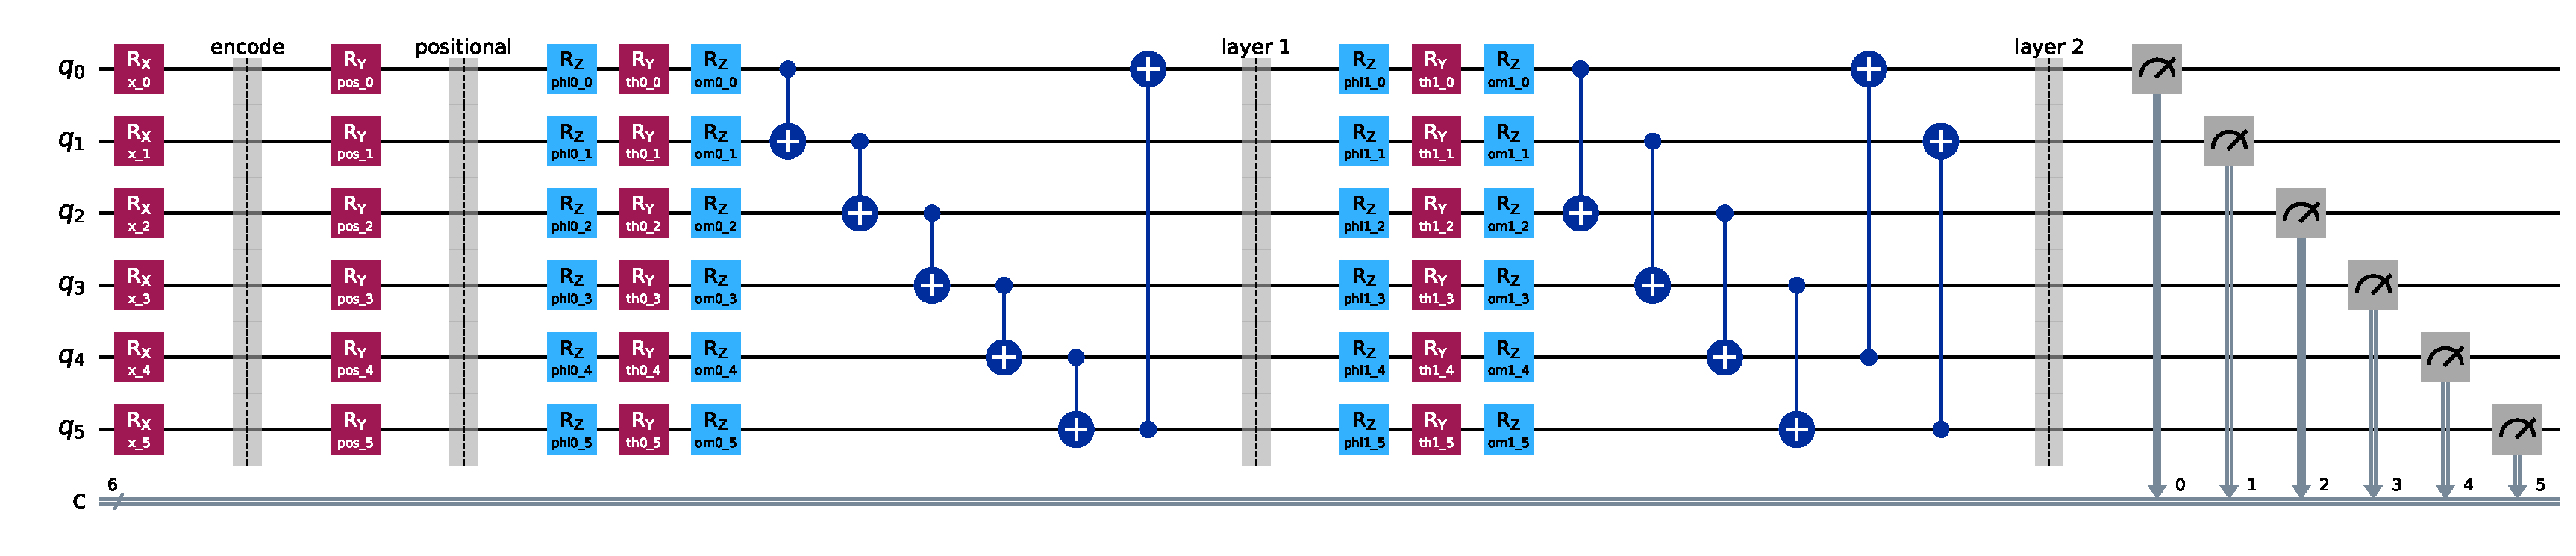
\includegraphics[width=\textwidth]{figures/hvk1d_ansatz.pdf}\\[6pt]
  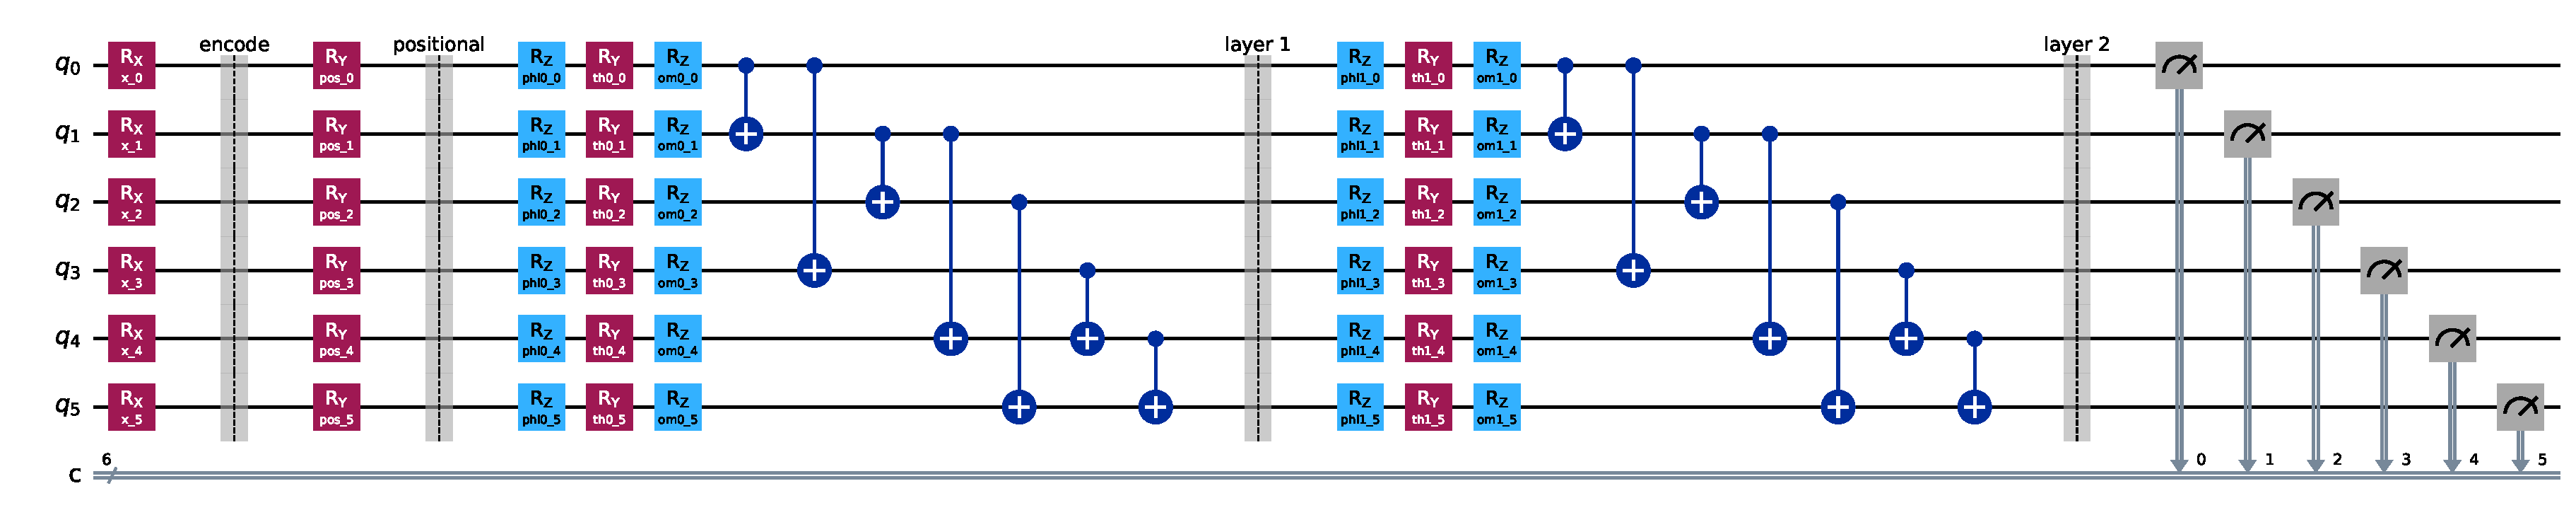
\includegraphics[width=\textwidth]{figures/hvk2d_ansatz.pdf}
  \caption{The PCAE1D (top) and PCAE2D (bottom) variational ans\"atze, exactly as
           executed (encoding $R_X$ rotations, positional $R_Y$ rotations, then
           two entangling layers of $R_Z$-$R_Y$-$R_Z$ single-qubit rotations with
           a CNOT ring for PCAE1D or fixed grid-edge CNOTs for PCAE2D). Both
           circuits were rebuilt gate-for-gate in Qiskit and validated against
           the original PennyLane training circuit before use in the hardware
           pilot of Section~\ref{sec:hardware_pilot}.}
  \label{fig:hvk_ansatz}
\end{figure}

Table~\ref{tab:variants} summarises the tested variants. PCAE1D uses a linear
6-qubit chain (5 nearest-neighbour bonds, 27-D observable vector); PCAE2D arranges
the same 6 qubits on a $2\times3$ lattice matching patch-boundary adjacency
(19-D latent signature); a symmetric PCAE1D variant adds a
$\mathrm{U}(1)$-preserving coupling constraint; and a $D_4$-pooled PCAE2D variant
(Section~\ref{sec:symmetry}) group-averages the observable grid over the eight
symmetries of the \del{square} \add{$4\times4$ patch grid},
$\Phi_{D_4}(x)=\tfrac{1}{8}\sum_{g\in D_4}P_g^{-1}\Phi(gx)$, which is equivariant
by construction. The IBM Cloud circuit probe reported in the supplement confirms
both PCAE1D and PCAE2D compile to depth-18, 6-qubit circuits on a Heron-class
basis.
\color{black}

\begin{table}[t]
  \centering
  \caption{PCAE variants tested in this paper.}
  \label{tab:variants}
  \begin{tabular}{@{}l l c l@{}}
    \toprule
    Variant                 & Topology                  & Latent dim. & Symmetry \\
    \midrule
    PCAE1D                   & 6-qubit chain             & 27-D        & None (control)            \\
    PCAE2D                   & $2\times3$ grid           & 19-D        & $D_4$-motivated only      \\
    Symmetric PCAE1D         & 6-qubit chain             & 27-D        & $\mathrm{U}(1)$ coupling  \\
    $D_4$-pooled PCAE2D      & $2\times3$ grid, pooled   & 19-D        & $D_4$-equivariant (exact) \\
    \bottomrule
  \end{tabular}
\end{table}

\section{Experimental Setup}
\label{sec:protocol}

\color{green}
\del{All image-reconstruction results in
Sections~\ref{sec:sameset_results}--\ref{sec:hardware_pilot} use the single-image
\textit{Monalisa} protocol developed for PCAE: a fresh model is optimised directly
on its target image, with no held-out split.} \add{The reconstruction results in
Sections~\ref{sec:sameset_results}, \ref{sec:no_generalization} and
\ref{sec:hardware_pilot}--\ref{sec:hardware_anchors} use the single-image
\textit{Monalisa} protocol developed for PCAE. A fresh model is optimised
directly on its target image, with no held-out split.} These results therefore measure
per-image fitting and reconstruction capability. The hardware pilot replays the
resulting fitted checkpoints on real devices without retraining. The symmetry
and \del{restricted-entanglement} \add{restricted pair-observable} diagnostics use the separate protocols stated in
their respective sections. The training-dynamics
readouts of Section~\ref{sec:phase_transition} are reported as an
interpretability diagnostic, with their scope set by the negative control given
there. Held-out generalisation and component necessity are evaluated under the
resource-matched statistical protocol of the companion supplementary study
(Section~\ref{sec:ablation_relationship}). All settings report MSE and
PSNR $=20\log_{10}(1/\sqrt{\mathrm{MSE}})$; image settings
additionally report SSIM. Full implementation settings and environment versions
are given in the companion supplementary document.
\color{black}

\section{Results}
\label{sec:results}

\color{blue}
\subsection{Reconstruction across six real image datasets}
\label{sec:sameset_results}

For each image, we trained a fresh PCAE2D model using non-overlapping $8\times8$
patches (16 patches/image, 80--100 optimisation steps). The sample covers
CIFAR-10 \citep{Krizhevsky2009}, MNIST \citep{LeCun1998}, Fashion-MNIST
\citep{Xiao2017}, and the PathMNIST, BloodMNIST, and PneumoniaMNIST subsets of
MedMNIST~v2 \citep{Yang2023}. Table~\ref{tab:sameset_multi_dataset} reports mean
PSNR between $25.8$ and $41.6$~dB (SSIM $0.91$--$1.00$). This establishes that
the architecture fits varied image structures under a common protocol.
\add{This protocol is per-image fitting, in the same sense as implicit neural
representations, which fit one network to one image
\citep{Sitzmann2020, Strumpler2022}. These results therefore measure
representation capacity. Generalisation to held-out images is tested in
Section~\ref{sec:ablation_relationship}. A compression claim would also need a bit
rate, which we do not report \citep{Strumpler2022}.}

\begin{table}[t]
  \centering
  \caption{PCAE2D same-set reconstruction across six real image datasets
           (per-image trained, 80--100 steps, mean $\pm$ std over sampled
           images).}
  \label{tab:sameset_multi_dataset}
  \begin{tabular}{@{}l c r@{\,$\pm$\,}l r@{\,$\pm$\,}l@{}}
    \toprule
    Dataset          & $n$ images & \multicolumn{2}{c}{PSNR (dB)} & \multicolumn{2}{c}{SSIM} \\
    \midrule
    CIFAR-10         & 3 & 37.75 & 2.38 & 0.9986 & 0.0003 \\
    MNIST            & 3 & 25.77 & 2.23 & 0.9783 & 0.0116 \\
    Fashion-MNIST    & 3 & 34.55 & 3.05 & 0.9980 & 0.0006 \\
    PathMNIST        & 3 & 36.86 & 2.11 & 0.9118 & 0.0627 \\
    BloodMNIST       & 2 & 36.57 & 2.36 & 0.9922 & 0.0063 \\
    PneumoniaMNIST   & 2 & 41.60 & 0.98 & 0.9985 & 0.0006 \\
    \bottomrule
  \end{tabular}
\end{table}



\subsection[Scope of per-image fitting]{\del{Scope: models do not transfer zero-shot} \add{Scope of per-image fitting}}
\label{sec:no_generalization}

\del{A model optimised on one image alone does not transfer zero-shot to a
structurally different image.} \add{A model optimised on one image is specific
to that image.} On \textit{Monalisa}, zero-shot transfer to a
second image reaches $8.31$~dB PSNR, with SSIM $0.1044$. Extending training to
include the second image recovers $28.63$~dB, with SSIM $0.9858$. The per-image
results above therefore measure per-image optimisation and reconstruction
capability. Section~\ref{sec:ablation_relationship} tests the held-out case
directly.

\color{black}

\subsection{Competitive with resource-matched classical baselines}
\label{sec:ablation_relationship}
\color{green}
The results above measure per-image fitting. A separate question is whether
PCAE's feature map improves reconstruction on real, \emph{held-out} images under
a resource-matched multi-seed protocol. \del{That question is answered in} \add{The full study is in} the
companion document, \textit{Supplementary Material for the Hamiltonian Vision
Kernel: Resource-Matched Ablations, Validation, and Reproducibility}. \add{Its
main results are summarised below, including the equivalence tests of
Table~\ref{tab:tost_main}.}

On held-out CIFAR-10, \snew{the raw/local linear control} reaches
$18.80\pm1.42$~dB, against PCAE2D's $18.12\pm1.54$~dB. Aggregating held-out
images within each split gives a PCAE2D-minus-control difference of $-0.68$~dB,
with bootstrap 95\% CI $[-0.91,-0.46]$~dB and Wilcoxon $p=0.0625$ at $n=5$
seeds. The same numerical direction holds on five further real datasets. The
tested PCAE map is therefore informative, \del{but it is not shown to outperform the
simpler maps on ordinary held-out reconstruction} \add{and on ordinary held-out
reconstruction it stays within 1~dB of the simpler maps}.

\add{All controls are matched at the readout. Each passes a 32-D feature vector
to the same linear readout with 2112 parameters, on the same splits. This
matches the readout resources. It does not match the feature class or the
compute cost. The controls differ in what their features can express. The
no-entanglement and $ZZ$-only controls remove all or part of the entangling
pair channel, and the quadratic classical control adds second-order classical
terms. The compute needed to produce the features is not matched, since PCAE2D
evaluates a quantum circuit for every patch.}
{\color{red}\textbf{[Student: (1) the held-out PCAE2D map is 32-D with 6 pair
channels (Supplement, Table~S-resource\_capacity), not the 19-D map of
Table~\ref{tab:configurations}. Please state this in both documents. (2) The
supplement never defines the quadratic classical control. Please add its
definition and confirm ``second-order classical terms''.]}}

A TOST equivalence test \add{\citep{Schuirmann1987, Lakens2017}} at a declared $\pm1$~dB margin confirms that this gap is
small enough\del{, in a pre-declared and data-independent sense,} to call the two
\emph{competitive} rather than merely ``not shown to differ''.
\add{The estimand is the seed-level PCAE2D-minus-control PSNR difference,
averaged over held-out images within each seed. Equivalence requires both
one-sided tests to reject at $\alpha=0.05$. This is the same as the 90\%
confidence interval lying inside $[-1,+1]$~dB (Table~\ref{tab:tost_main}). The
margin is a declared choice.}
{\color{red}\textbf{[Student: please decide on these three sentences. They are
not in the supplement, so add them only if you agree. (1) With five seeds,
$p=0.0625$ is the smallest two-sided Wilcoxon $p$-value possible, so the
Wilcoxon test cannot reach $0.05$. (2) The $t$-based 90\% interval is wider than
the bootstrap 95\% interval, because with only five seeds the bootstrap interval
tends to be too narrow. (3) A 1~dB change in PSNR is a factor of about $1.26$ in
MSE.]}}
{\color{red}\textbf{[Student: when was the $\pm1$~dB margin fixed? If a dated
commit shows it was set before the TOST run, cite it in the supplement. If not,
remove ``pre-declared'' from the abstract, contribution~3 and the conclusion.
The supplement's current reason for the margin uses the observed 3--7~dB gaps,
which makes it depend on the data.]}}
\snew{Five of seven distinct} tested controls \del{are statistically equivalent to}
\add{meet the equivalence criterion against} PCAE2D within that margin. The two weakest controls, strict classical random
features and random-VQC, are correctly excluded, because PCAE2D substantially
outperforms them. \add{Each control is tested separately at $\alpha=0.05$, with
no correction for the seven comparisons.}
{\color{red}\textbf{[Student: the seven TOST tests are not corrected for
multiple comparisons. Under a Holm correction, four equivalences would stay (no
entanglement, $ZZ$-only, quadratic classical, shuffled pair observables). The
raw/local linear control ($p=0.034$), which the abstract names, would not pass.
Please choose one with the PI. (a) Keep the uncorrected tests and say so in the
abstract. (b) Name a different control in the abstract. (c) Run and report a
corrected analysis yourself.]}}

\begin{table}[t]
  \centering
  \caption[TOST equivalence test on held-out CIFAR-10]{\add{TOST equivalence
           test on held-out CIFAR-10 ($\pm1$~dB margin, $\alpha=0.05$, five
           seed-level paired differences, PCAE2D minus control). Equivalence
           requires the 90\% CI to lie inside $[-1,+1]$~dB. Values from the
           Supplementary Material.}}
  \label{tab:tost_main}
  \footnotesize\bfseries
  \setlength{\tabcolsep}{3.5pt}
  \begin{tabular}{@{}l r c r l@{}}
    \toprule
    Control                          & $\Delta$PSNR (dB) & 90\% CI (dB)       & TOST $p$  & Verdict \\
    \midrule
    Raw/local linear                 & $-0.68$ & $[-0.96,-0.40]$ & $0.034$   & Equivalent \\
    No entanglement                  & $-0.34$ & $[-0.69,+0.02]$ & $0.008$   & Equivalent \\
    $ZZ$-only observables            & $-0.44$ & $[-0.61,-0.27]$ & $0.001$   & Equivalent \\
    Quadratic classical              & $-0.21$ & $[-0.46,+0.03]$ & $0.001$   & Equivalent \\
    Shuffled pair observables        & $-0.19$ & $[-0.35,-0.02]$ & $<0.001$  & Equivalent \\
    Strict classical random features & $+2.27$ & $[+1.92,+2.63]$ & $0.999$   & PCAE2D better \\
    Random VQC                       & $+6.97$ & $[+5.56,+8.39]$ & $1.000$   & PCAE2D better \\
    \bottomrule
  \end{tabular}
\end{table} We report this as a complement to the positive \del{entanglement} \add{pair-observable}
and symmetry results below. It delineates their tested boundary and records the
provenance checks that prevented exploratory artifacts from becoming claims.

A matched-budget, multi-seed rerun of the component-ablation table reaches the
same conclusion on ordinary per-image reconstruction. The rerun uses 240 steps
and 3 seeds per variant. {\color{red}\textbf{It replaces an earlier table that
we withdrew, because the repository does not retain the per-seed records needed
to reproduce it.}} A plain classical-replacement control ties or slightly
exceeds the quantum baseline, and only a circuit-free random-VQC control
performs clearly worse. This rerun uses a descriptive pooled-standard-deviation
comparison rule at 3 seeds rather than a calibrated test, and full results are in
the companion supplement. Section~\ref{sec:dequant} discusses why this
ties-with-classical result and the \del{entanglement-necessity}
\add{pair-observable necessity} result of
Section~\ref{sec:entanglement_necessity} are \del{not in tension} \add{consistent}.


\subsection{A real hardware reconstruction pilot}
\label{sec:hardware_pilot}

The results above are noiseless-simulator results. We now report a small but
complete image-reconstruction pilot executed on real IBM Quantum hardware
(\texttt{ibm\_fez}, a 156-qubit Heron-class processor), going beyond the
compiled-circuit feasibility probe documented in the supplement.

The pilot covers five images. These are the full 16-patch \textit{Monalisa}
benchmark and four native-resolution CIFAR-10 images (\textit{cat},
\textit{ship}$\times2$, \textit{airplane}), each optimised directly on its own
target image following the same per-image protocol as \del{every result in this
paper} \add{Sections~\ref{sec:sameset_results} and~\ref{sec:no_generalization}}. For each image we took an already-trained PCAE1D/PCAE2D checkpoint's exact
learned parameters and rebuilt its measurement circuits gate-for-gate in Qiskit.
We verified the translation against the original PennyLane simulator to within
numerical noise, at most $7.9\times10^{-4}$ maximum absolute error per
observable across every patch, with full validation numbers in the companion
supplementary document. We then executed the same circuits on real hardware with
256 shots per measurement basis. This is a fixed per-basis shot budget, rather
than an adaptive shadow-tomography-style estimation scheme
\citep{Huang2020Shadows}. The hardware-measured observables were decoded by the
same trained classical decoder, with no retraining and no simulator involved
anywhere in the reconstruction path.

Reconstructions from real, noisy hardware measurements retain recognisable image
structure. \textit{Monalisa} reaches $25.90$~dB PSNR from hardware measurements,
against a $37.99$~dB noiseless-simulator replay of the identical circuit
(Figure~\ref{fig:hardware_reconstruction_monalisa}). The four CIFAR-10 images
average $29.56\pm2.03$~dB on hardware against $42.69\pm3.84$~dB in simulation
(Figure~\ref{fig:hardware_reconstruction_cifar},
Table~\ref{tab:hardware_pilot_summary}). The observed gap is consistent with
noise in these unmitigated device executions, although the five-image pilot does
not isolate individual noise sources.
{\color{red}\textbf{[Student: the text calls these runs unmitigated. Please
state (1) which error-suppression and mitigation options were switched off in
SamplerV2, for example dynamical decoupling and twirling, (2) the date and time
of the calibration data, (3) which physical qubits were used on each backend,
and (4) the total number of shots per image. The supplement already gives the
optimisation level, circuit depth, CX count and job IDs.]}} Every hardware reconstruction remains above
the random-latent control range ($11$--$15$~dB in the companion supplementary
study). The pilot used 176 circuits; the contemporaneous account-meter reading
increased by 16 quantum-processor seconds, with the provenance limitation
documented in the supplement.

\begin{table}[t]
  \centering
  \caption{Real IBM hardware reconstruction pilot (backend \texttt{ibm\_fez},
           256 shots/basis, no retraining). PSNR compares hardware-decoded and
           simulator-decoded reconstructions against the same ground-truth
           image.}
  \label{tab:hardware_pilot_summary}
  \begin{tabular}{@{}l c c c@{}}
    \toprule
    Image                              & Patches & Sim.\ PSNR (dB)   & HW PSNR (dB)      \\
    \midrule
    Monalisa (PCAE1D)                   & 16      & 37.99             & 25.90             \\
    CIFAR cat (PCAE2D)                  & 16      & 44.85             & 31.52             \\
    CIFAR ship, hydrofoil (PCAE2D)      & 16      & 36.56             & 26.44             \\
    CIFAR ship, sea boat (PCAE2D)       & 16      & 42.57             & 31.20             \\
    CIFAR airplane (PCAE2D)             & 16      & 46.79             & 29.10             \\
    \midrule
    CIFAR mean $\pm$ std (4 images)    & ---     & $42.69\pm3.84$    & $29.56\pm2.03$    \\
    \bottomrule
  \end{tabular}
\end{table}

\begin{figure}[t]
  \centering
  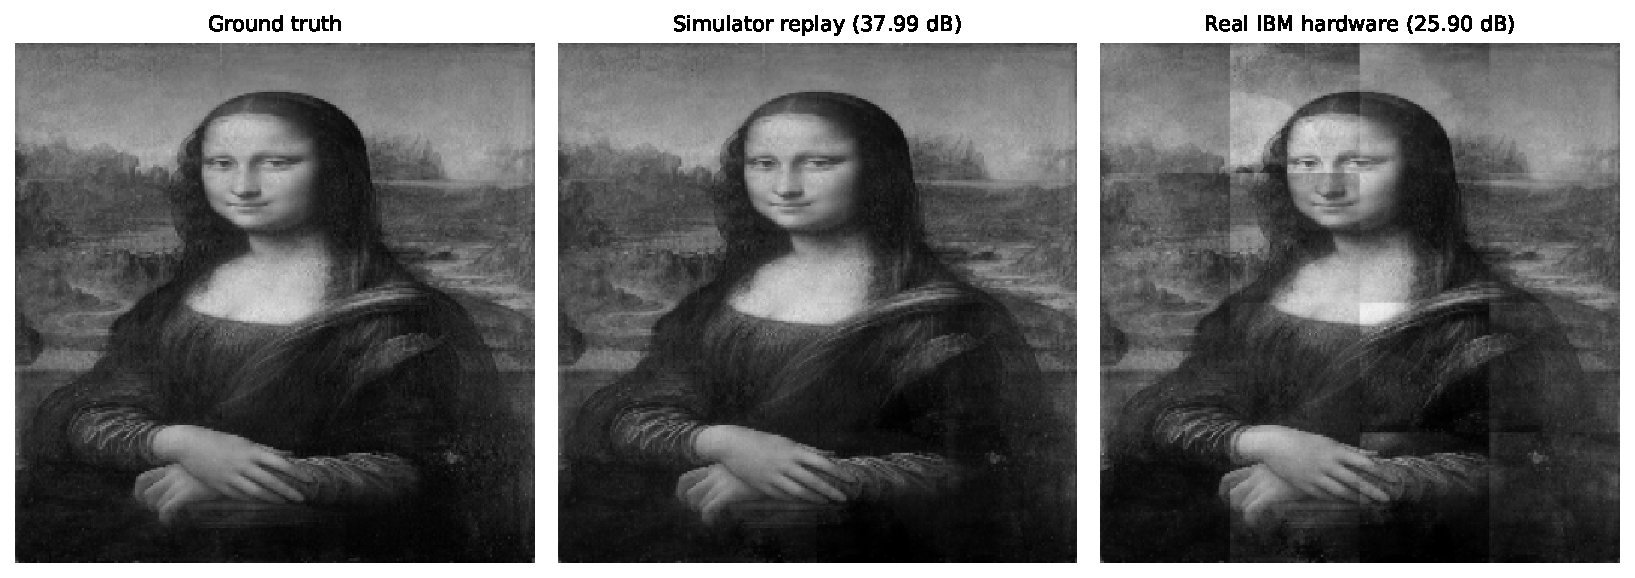
\includegraphics[width=\textwidth]{figures/ibm_hardware_reconstruction_monalisa.pdf}
  \caption{\textit{Monalisa} reconstructed from real IBM Quantum hardware
           measurements (right) against the same trained checkpoint's
           noiseless-simulator replay (centre) and ground truth (left). The
           hardware image is visibly noisier and exhibits patch-boundary banding,
           while the subject remains recognisable.}
  \label{fig:hardware_reconstruction_monalisa}
\end{figure}

\begin{figure}[t]
  \centering
  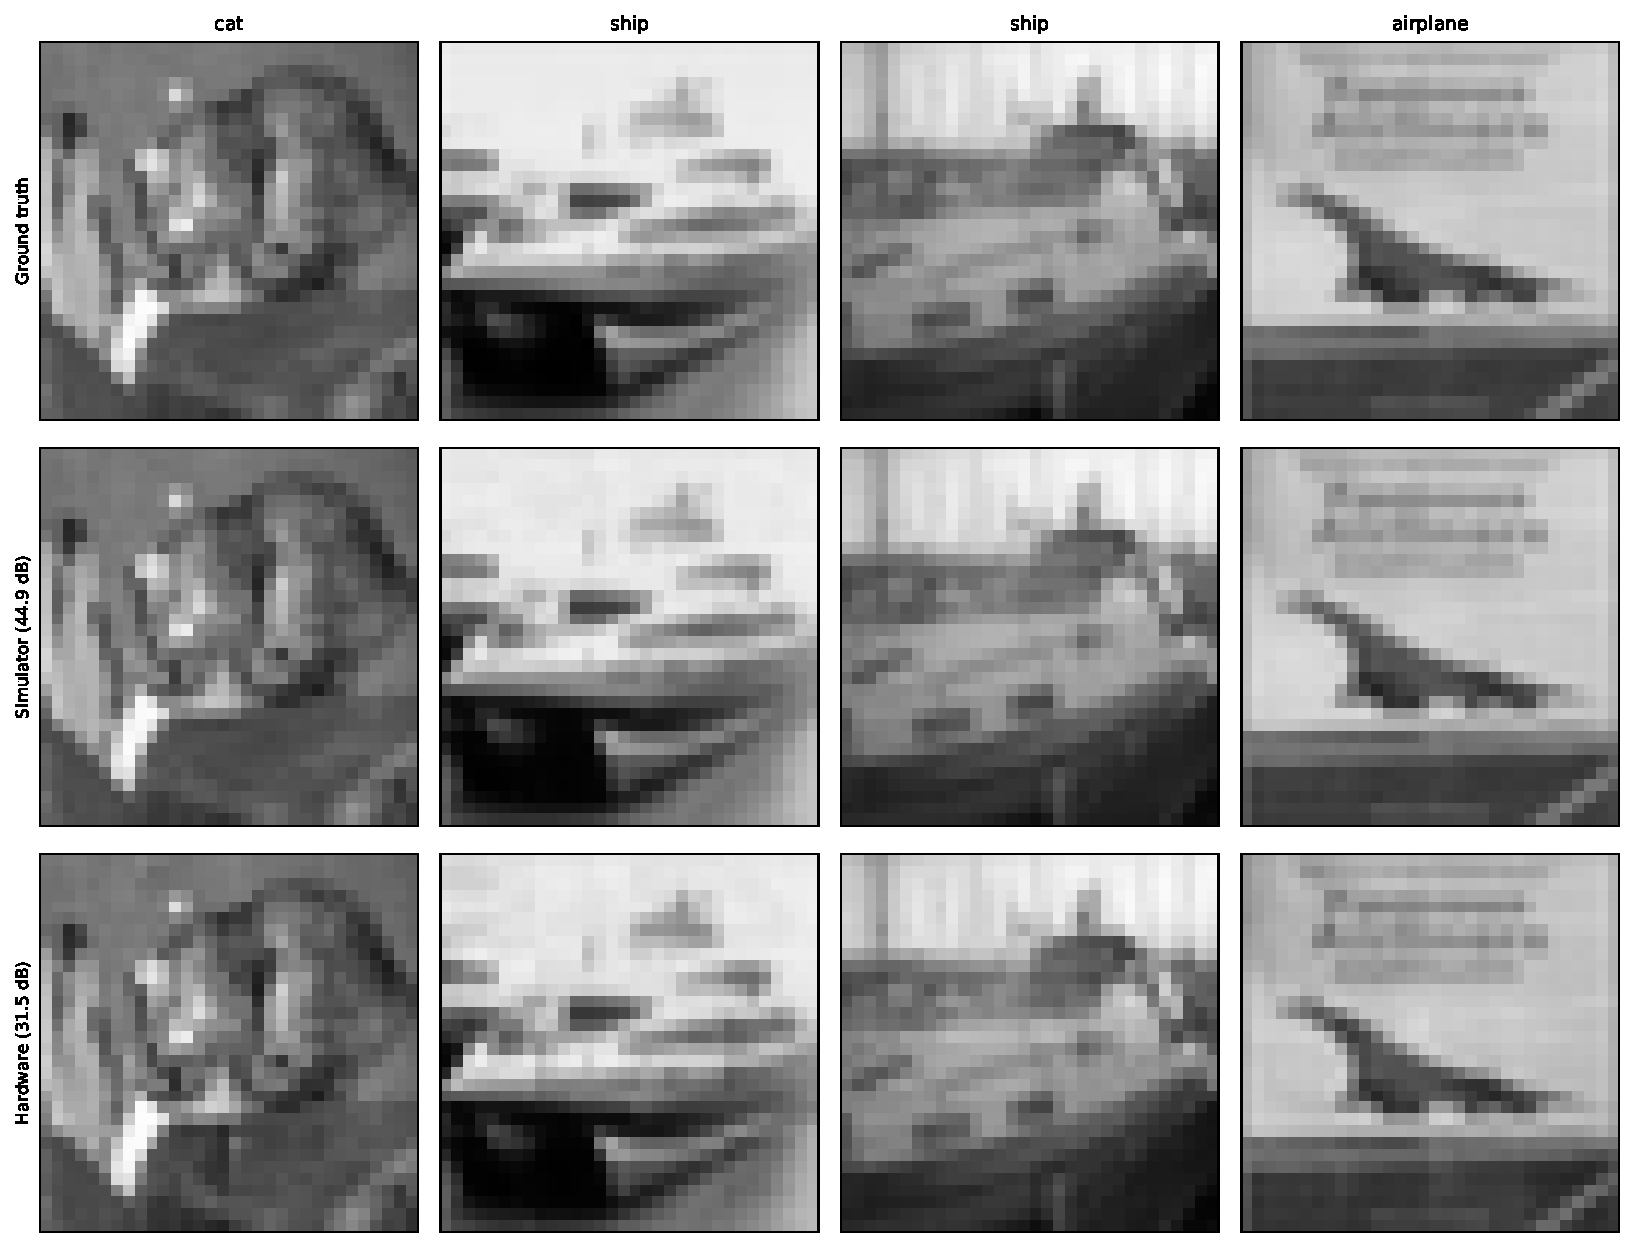
\includegraphics[width=\textwidth]{figures/ibm_hardware_reconstruction_cifar.pdf}
  \caption{Four CIFAR-10 images reconstructed from real IBM Quantum hardware
           measurements (bottom row) against noiseless-simulator replays of the
           same trained PCAE2D checkpoints (middle row) and ground truth (top
           row).}
  \label{fig:hardware_reconstruction_cifar}
\end{figure}

\del{Five images constitute a pilot, and we make no hardware-advantage claim. What
the pilot does establish is that} \add{The pilot establishes that} the trained PCAE observable channel survives
execution on present-day hardware. \add{With five images it is a pilot, and it
makes no hardware-advantage claim.} The learned parameters, the measurement
circuits and the classical decoder all transfer unchanged, and the decoded
images remain quantitatively informative at 256 shots per basis on an
unmitigated device. This is the sense in which PCAE runs on real quantum
hardware. The companion supplementary document gives the full methodology,
covering exact gate sequences, per-basis measurement construction, job IDs, and
pre-submission local-validation results.

The same checkpoint-replay methodology supports a further \del{hardware-validation
exercise} \add{hardware replay}, reported in the companion Supplementary Material. Fresh PCAE1D
checkpoints were trained at $N\in\{4,6,8\}$ and replayed epoch-by-epoch on real
IBM Quantum hardware and on the IonQ cloud simulator \citep{IonQBackends}. That
exercise serves the training-dynamics diagnostic of
Section~\ref{sec:regularizer_inert}. {\color{red}\textbf{It stays out of the
main text because it is a single-patch, single-seed probe, and because the
threshold it tracks fires equally with the Hamiltonian term present and absent
(Section~\ref{sec:phase_transition}). We therefore treat it as an
interpretability readout, on the same footing as the traces it supports.}}
{\color{red}\textbf{[Student: this paragraph says the hardware replay serves the
training-dynamics diagnostic of Section~\ref{sec:regularizer_inert}. That
diagnostic is reported in Section~\ref{sec:phase_transition}. Please confirm
which section is meant.]}}
\color{black}


\subsection{Noise/shot trade-off: a free simulator complement}
\label{sec:hardware_robustness}

\color{blue}
The five-image pilot above used a single shot budget (256/basis) and one
execution per image, which bounds how much it can say about noise sensitivity on
its own. \del{Real IBM Quantum time is a scarce free-tier resource, so we separate} \add{To use IBM Quantum time well, we separate}
what a \emph{calibrated device-noise simulation} can establish at zero hardware
cost from what genuinely requires hardware. Using \texttt{qiskit-aer} with the
live calibration snapshot of \texttt{ibm\_fez} (\texttt{FakeFez}, no
quantum-processor time consumed), we replay the same already-trained
checkpoints' circuits at four shot budgets (256/512/1024/4096 shots per basis,
three repeated executions each) and compare against both the noiseless-simulator
ceiling and the real-hardware point already reported above.



\begin{figure}[t]
  \centering
  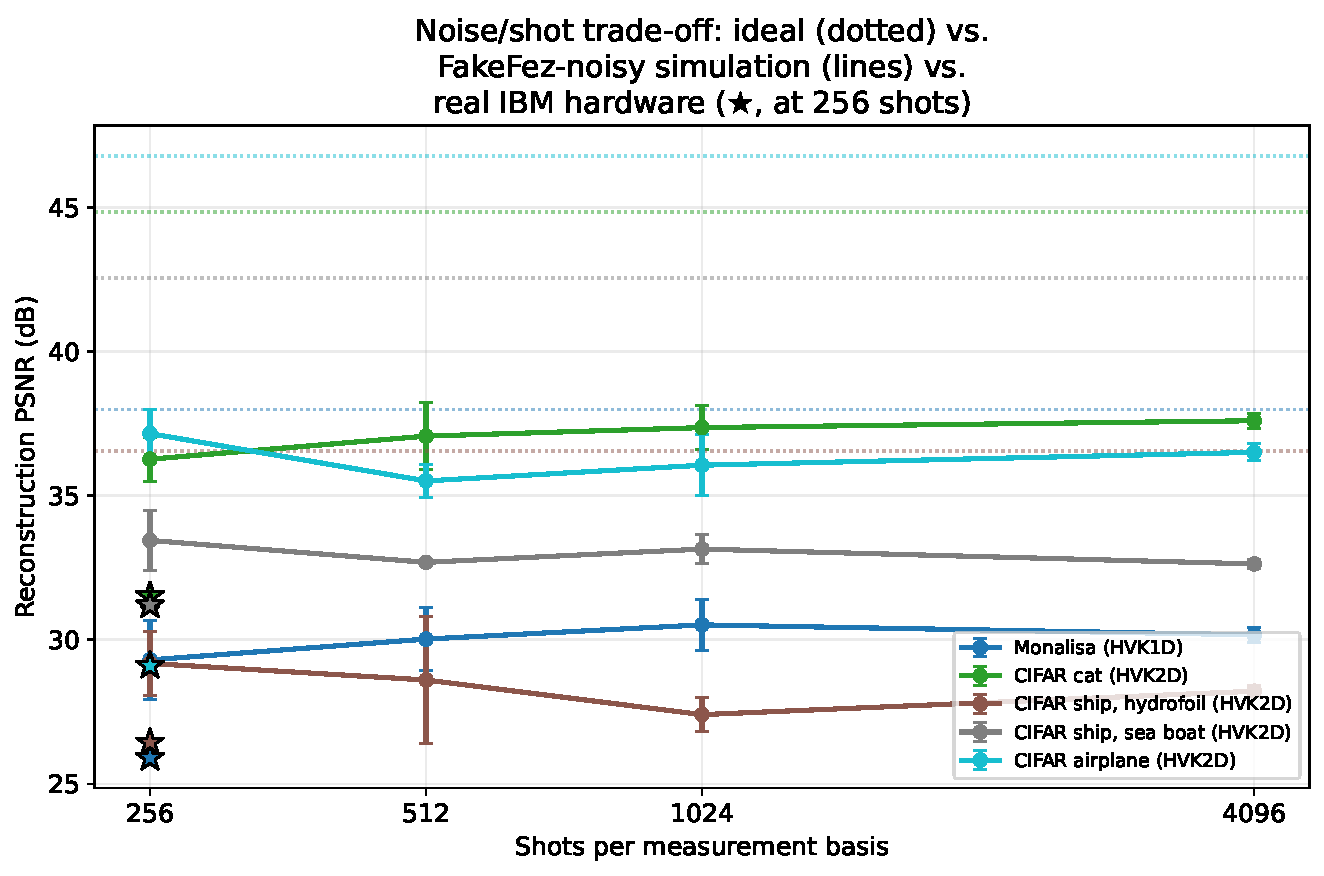
\includegraphics[width=0.85\textwidth]{figures/hardware_robustness_shot_sweep.pdf}
  \caption{Calibrated device-noise simulation (\texttt{FakeFez}, mean $\pm$ std
           over three executions). Dotted lines show noiseless ceilings and stars
           show real-hardware measurements. Increasing 256 to 4096 shots changes
           mean PSNR by only $-0.05$~dB.}
  \label{fig:hardware_robustness_shot_sweep}
\end{figure}

Two findings follow, averaged over the five checkpoints. First, shot noise
accounts for only part of the noiseless-to-real gap. Moving from the noiseless
ceiling to a calibrated-noise simulation at the same 256-shot budget already
costs $8.68$~dB on average, before any real device is involved. Second, more
shots \del{does} \add{do} not reliably recover it. Increasing to 4096 shots per basis changes
PSNR by only $-0.05$~dB on average across the five checkpoints, with individual
images ranging from a $1.33$~dB gain to a $0.96$~dB loss. At this circuit size
and shot range, shot count is not a lever that reliably improves reconstruction
quality.
\color{green}

Comparing the 256-shot noisy simulation directly against the real-hardware point
isolates what the calibration snapshot does \emph{not} capture. That comparison
leaves a further $4.24$~dB average gap, ranging from $2.25$ to $8.06$~dB across
images. \del{We attribute this residual to} \add{This residual is consistent
with effects that the calibration model does not capture, such as} drift between calibration and execution,
crosstalk, and correlated errors. \add{The pilot does not separate these
sources.} The airplane image is the clear outlier, with
an $8.06$~dB residual gap, roughly double any other image. We report it rather
than exclude it, since a single-execution, five-image pilot cannot distinguish an
image-specific effect from ordinary job-to-job variation. This calibrated-noise
simulation is a free, repeatable complement to the pilot, not a substitute for
it. It bounds how much of the observed hardware gap is attributable to modelled
device noise rather than unmodelled effects, using zero additional
quantum-processor time.
\color{black}

\subsection{Real-hardware anchor points: repeated execution and a second backend}
\label{sec:hardware_anchors}

\del{The simulated trade-off above is bounded, in turn, by whether it actually
reflects real devices. We confirmed this directly on hardware, using a small,
quota-tracked slice of the free-tier IBM Quantum allowance of four jobs, well
under $1\%$ of the monthly limit.} \add{The simulated trade-off above is useful
only if it reflects real devices. We checked this directly on hardware with four
jobs from the free-tier IBM Quantum allowance. These four jobs used well under
$1\%$ of the monthly limit.} Two checkpoints, \textit{Monalisa} and CIFAR
\textit{cat}, were replayed with no retraining on \texttt{ibm\_marrakesh} and
\texttt{ibm\_kingston}. Both backends are distinct from the original pilot's
\texttt{ibm\_fez}. We ran them at the original 256-shot budget and, separately,
at 1024 shots.

\begin{table}[t]
  \centering
  \caption{Real-hardware anchor points: same checkpoints, no retraining, on two
           further backends. The original pilot's \texttt{ibm\_fez} point is
           shown for reference.}
  \label{tab:hardware_anchors}
  \begin{tabular}{@{}l l r r@{}}
    \toprule
    Image       & Backend                       & Shots & PSNR (dB) \\
    \midrule
    Monalisa    & \texttt{ibm\_fez} (original)  &  256  & 25.90     \\
    Monalisa    & \texttt{ibm\_marrakesh}       &  256  & 25.94     \\
    Monalisa    & \texttt{ibm\_kingston}        & 1024  & 26.10     \\
    \addlinespace
    CIFAR cat   & \texttt{ibm\_fez} (original)  &  256  & 31.52     \\
    CIFAR cat   & \texttt{ibm\_kingston}        &  256  & 28.93     \\
    CIFAR cat   & \texttt{ibm\_kingston}        & 1024  & 31.24     \\
    \bottomrule
  \end{tabular}
\end{table}

\textit{Monalisa} reproduces almost exactly across backends at matched shots
($25.94$ vs.\ $25.90$~dB, \texttt{ibm\_marrakesh} vs.\ \texttt{ibm\_fez}), and
gains only $0.16$~dB from quadrupling shots to 1024, consistent with the
simulated finding above that shot count is not a reliable lever. The CIFAR
\textit{cat} point is the more informative one. On \texttt{ibm\_kingston} at the
original 256-shot budget it reaches $28.93$~dB, which is $2.59$~dB below the
\texttt{ibm\_fez} pilot point. Its own 1024-shot execution on the same backend
recovers to $31.24$~dB, within $0.28$~dB of the original. This is real
job-to-job and backend-to-backend variation of a magnitude comparable to the
unmodelled residual identified by the simulator comparison
(Section~\ref{sec:hardware_robustness}). \del{It provides direct evidence, not merely
a simulated bound, that a single 256-shot execution on a single backend is not
yet a stable estimate of this pipeline's hardware performance, and that repeated
execution matters at least as much as backend choice or shot count individually.}
\add{It gives direct evidence that repeated execution matters at least as much as
backend choice or shot count. A single 256-shot run on one backend is not yet a
stable estimate of hardware performance.}

\subsection{Exact \texorpdfstring{$D_4$}{D4}-equivariant observable pooling}
\label{sec:d4}
\label{sec:symmetry}

A $D_4$-pooled PCAE2D observable-grid map is equivariant to the eight symmetries
of the square \emph{by construction}:
\begin{equation}
  \Phi_{D_4}(x)=\frac{1}{8}\sum_{g\in D_4}P_g^{-1}\Phi(gx),
  \qquad
  \Phi_{D_4}(hx)=P_h\,\Phi_{D_4}(x)\ \ \forall\, h\in D_4,
\end{equation}
\del{up to floating-point error. We verify this numerically} \add{Here $D_4$
acts on an image $x$ by rotating or reflecting its $4\times4$ grid of patches,
and $P_g$ permutes the per-patch observable vectors in the same way, so that
$P_{gh}=P_gP_h$. The property then holds exactly for any base map $\Phi$.
Substituting $hx$ and re-indexing the sum with $g'=gh$ gives
$P_g^{-1}=P_hP_{g'}^{-1}$, and hence $\Phi_{D_4}(hx)=P_h\Phi_{D_4}(x)$. The
numerical check below therefore tests the implementation, not the property. We
run it} over 7000 patch
transforms of cached CIFAR images (Table~\ref{tab:d4_equivariance},
Figure~\ref{fig:d4_equivariance}). The pooled map's equivariance error is
$9.57\times10^{-17}\pm1.26\times10^{-17}$, which is floating-point noise. The
unpooled positional map has an error of $0.815\pm0.129$, and the local/raw
control has $0.837\pm0.131$. Both are of order one. The patch grid's geometry
therefore makes the unpooled map $D_4$-\emph{motivated} only, and the explicit
pooling construction is what delivers the property. This construction operates
at the feature-grid level and serves here as a numerical diagnostic, rather
than as a component of the trainable reconstruction pipeline. Integrating it
end-to-end (Section~\ref{sec:limitations}) is concrete future work.
\add{This route to symmetry differs from equivariant quantum neural networks,
in which every circuit layer is built to commute with the group action
\citep{Nguyen2024EQNN}. A recent image classifier of that kind builds $C_4$
rotation symmetry into the circuit itself \citep{SanSebastianSein2025}. In PCAE
the symmetry comes from averaging the observable grid over the group after
measurement. The circuit itself is not equivariant, and the same average applies
equally to a classical feature map.}
{\color{red}\textbf{[Student: Table~\ref{tab:d4_equivariance} labels the second
column ``Std.\ error'', but the text reads it as a standard deviation over 7000
transforms. Please confirm which it is and fix the header.]}}

\begin{table}[t]
  \centering
  \caption{$D_4$ equivariance error for unpooled and pooled observable-grid maps
           (lower is better; the pooled map is group-averaged over all eight
           square symmetries).}
  \label{tab:d4_equivariance}
  \begin{tabular}{@{}l r r@{}}
    \toprule
    Model                    & Mean error              & Std.\ error             \\
    \midrule
    $D_4$-pooled PCAE2D       & $9.57\times10^{-17}$    & $1.26\times10^{-17}$    \\
    No positional encoding   & $7.40\times10^{-1}$     & $1.52\times10^{-1}$     \\
    PCAE2D positional         & $8.15\times10^{-1}$     & $1.29\times10^{-1}$     \\
    Local/raw                & $8.37\times10^{-1}$     & $1.31\times10^{-1}$     \\
    \bottomrule
  \end{tabular}
\end{table}

\begin{figure}[t]
  \centering
  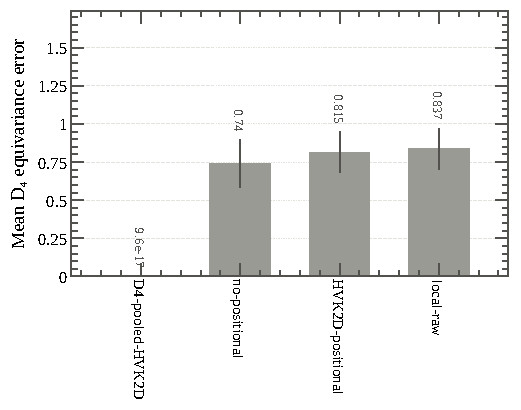
\includegraphics[width=0.85\textwidth]{figures/d4_equivariance_summary.pdf}
  \caption[$D_4$ equivariance diagnostic]{$D_4$ equivariance diagnostic. \del{The unpooled positional map is not
           equivariant; the group-pooled map is equivariant to numerical
           precision.} \add{The group-pooled map is equivariant to numerical
           precision. The unpooled positional map is not.}}
  \label{fig:d4_equivariance}
\end{figure}

\subsection[Pair-observable necessity in the nonlocal-structure protocol]{\del{Entanglement} \add{Pair-observable} necessity in the nonlocal-structure protocol}
\label{sec:entanglement_necessity}

The diagnostic tests whether \del{an entangling} \add{a} pair-observable channel is needed to
fit a target that depends on pair correlations. The target is a fixed synthetic
function of \emph{simulated} patch features, and those features are not
concatenated into any candidate's own input block. The companion supplement
gives the leakage-audit procedure that rules out circularity. Every control
receives the same raw inputs as PCAE2D. {\color{red}\textbf{The task is by
construction favourable to pair-observable structure, which is why we read it as
a representational statement and not as a performance comparison.}}

Table~\ref{tab:hvk_pair_diagnostic} and Figure~\ref{fig:hvk_pair_diagnostic}
report the result across five seeds. PCAE2D's \del{entangling observable}
\add{pair-observable} channel
reaches mean $R^2=0.9735$, or $32.77$~dB PSNR. This is a $17.74$~dB improvement
over a no-entanglement control ($R^2=0.019$) and $18.52$~dB over random-VQC
latents ($R^2=-0.173$). Freezing the quantum circuit, so that features are fixed
and only the readout is trained, still reaches $R^2=0.853$. A parameter-matched
classical control ($R^2=-0.030$) and a frozen-classical control ($R^2=-0.903$)
fail outright. {\color{red}\textbf{The raw-linear classical control
($R^2=0.0133$) is in the table but is not named here; whether it should be
depends on the duplicate-control question raised separately.}}
{\color{red}\textbf{[Student: please state what the no-entanglement control
measures. If it still measures $ZZ$ on a product state, then
$\langle Z_iZ_j\rangle=\langle Z_i\rangle\langle Z_j\rangle$ exactly, and its
failure needs one sentence of explanation. If it drops the pair channel, its
name should be ``no pair observables''.]}}

The mechanism is explicit under the fixed linear readout. A linear map of
single-patch expectations $\{\langle O_i\rangle\}$ cannot form the cross-term
$\langle O_i\rangle\langle O_j\rangle$ that the target depends on. The \del{entangling}
\add{pair} measurement supplies the joint correlator $\langle O_iO_j\rangle$ directly as a
feature. \add{Formally, let $z_i=\langle O_i\rangle$ and let every admissible
predictor be affine, $f(z)=w^{\top}z+b$. Then
$\partial^2 f/\partial z_i\partial z_j=0$ for all $i,j$. A target with a term
$c\,z_iz_j$, $c\neq0$, has this mixed derivative equal to $c$ wherever $z_i$ and
$z_j$ vary independently, so no affine $f$ can fit it. Adding $z_iz_j$ to the
feature vector makes the term linearly representable.} \del{An entangling}
\add{A} pair-observable channel is therefore
\emph{representationally necessary within the tested feature class and fixed
linear-readout protocol} to fit this target. \del{A sufficiently nonlinear classical
readout could in principle recover the same cross-terms, which is why we scope}
\add{A classical model that forms the same products, for example through
quadratic features or a nonlinear readout, would also fit this target. For this
reason we scope} the claim to the linear protocol rather than to classical models in general.

\begin{table}[t]
  \centering
  \caption[PCAE2D restricted pair-correlation diagnostic]{PCAE2D restricted pair-correlation diagnostic across five seeds.
           Deliberately favourable to pair-observable structure; evidence for
           \del{entanglement-necessity} \add{pair-observable necessity} under a matched linear readout.}
  \label{tab:hvk_pair_diagnostic}
  \begin{tabular}{@{}l r r r@{}}
    \toprule
    Model                            & Mean MSE                  & Mean PSNR (dB) & Mean $R^2$ \\
    \midrule
    PCAE2D \del{entangling} \add{pair} observables     & $8.5969\times10^{-4}$     & 32.77          & $ 0.9735$  \\
    Freeze quantum                   & $4.7904\times10^{-3}$     & 27.34          & $ 0.8533$  \\
    No entanglement                  & $3.1461\times10^{-2}$     & 15.03          & $ 0.0191$  \\
    Raw-linear classical             & $3.1654\times10^{-2}$     & 15.00          & $ 0.0133$  \\
    Parameter-matched classical      & $3.3033\times10^{-2}$     & 14.82          & $-0.0297$  \\
    Random VQC                       & $3.7616\times10^{-2}$     & 14.25          & $-0.1732$  \\
    Freeze classical                 & $6.0973\times10^{-2}$     & 12.17          & $-0.9025$  \\
    \bottomrule
  \end{tabular}
\end{table}

\begin{figure}[t]
  \centering
  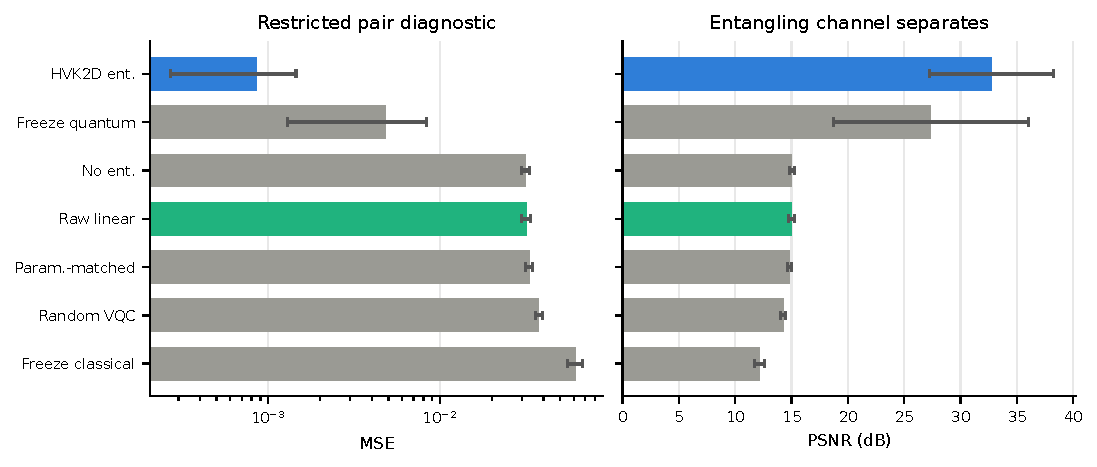
\includegraphics[width=0.9\textwidth]{figures/full_ablation_metric_comparison.pdf}
  \caption[Restricted pair-correlation diagnostic summary]{Restricted pair-correlation diagnostic summary (mean $\pm$ std over
           five seeds). The \del{entangling observable} \add{pair-observable} feature map dominates every
           control on this deliberately favourable task.}
  \label{fig:hvk_pair_diagnostic}
\end{figure}

\subsection{A scoped training-dynamics diagnostic}
\label{sec:phase_transition}

Beyond the results above, we tracked two exploratory training-dynamics readouts.
These are a magnetisation-style statistic $M_z(t)$ and a signed
energy-to-entanglement ratio $R_{ES}(t)$. Both drift smoothly over training with
run-to-run fluctuations, and neither shows a sharp transition. Any apparent onset
is a within-run median-plus-$2\sigma$ threshold crossing, rather than a
calibrated statistical test.

A negative control fixes the scope. We applied the identical protocol to a
classical-replacement variant, in which the Hamiltonian energy is identically
zero throughout training. That variant crosses the threshold in all $4/4$ tested
cases, which is as often as the Hamiltonian-regularised model's $4/4$. The
threshold therefore fires whether the Hamiltonian term is present or absent, and
it does not track that term. \del{We make no transition claim, and report} \add{We therefore report} these traces
as an interpretability readout on the learned energy and entanglement. The
companion Supplementary Material gives the full protocol and tables.

\section{Discussion}
\label{sec:discussion}

\subsection[Effect of the Hamiltonian energy term]{\del{Why the physics-informed regulariser was inert} \add{Effect of the Hamiltonian energy term}}
\label{sec:regularizer_inert}

Table~\ref{tab:hamiltonian_controls} shows the Hamiltonian energy term is a mild drag on reconstruction quality. The legacy objective adds a signed mean energy to the reconstruction loss. Because learned energy can go negative, the optimiser can lower total loss by driving energy down without improving reconstruction. Removing the term improves PSNR from $38.63$ to $44.56$~dB. A contrastive variant, assigning lower energy to correct feature--position pairs than to shuffled pairs, recovers part of the gap ($42.92$~dB) but stays below its no-energy counterpart. These are fresh same-environment measurements (\textit{Monalisa}, 200 steps, seed 42), and they supersede earlier values produced by a script that cannot be audited.

The learned couplings enter only the energy term and never reach the decoder. The Hamiltonian is therefore a \emph{read-only} observable of the trained representation rather than an inductive bias on reconstruction, and this is the sense in which we call it a diagnostic. A physically motivated regulariser has room to help when it resolves an otherwise underdetermined objective. This patch-level pixel task does not meet that condition, because the reconstruction loss already dominates the optimisation signal at this model scale. The Supplementary Material gives the full account.
{\color{red}\textbf{[Student: two points in this section. (1) The text calls
the Hamiltonian a read-only observable. But removing the energy term changes
PSNR from 38.63 to 44.56~dB (Table~\ref{tab:hamiltonian_controls}), so its
gradient does change the trained circuit, unless the energy is computed on
detached features. Please reword ``read-only''. (2) A gap of this size is more
than ``a mild drag''. Please choose wording that matches the table.]}}

\begin{table}[t]
  \centering
  \caption{Hamiltonian-sector controls (single-seed, fresh same-environment
           reproduction: \textit{Monalisa}, 200 steps, seed 42). The energy
           objective is diagnostically useful but does not improve reconstruction
           accuracy. See the Supplementary Material for the full reproducibility
           investigation and additional observable-sector controls.}
  \label{tab:hamiltonian_controls}
  \begin{tabularx}{\textwidth}{@{}L{0.30\textwidth} c Y@{}}
    \toprule
    Experiment                      & PSNR (dB) & Interpretation \\
    \midrule
    Legacy baseline, signed energy  & 38.63     & Standard energy-regularised run \\
    No energy loss                  & 44.56     & Removing energy improves PSNR \\
    Contrastive Hamiltonian core    & 42.92     & Stronger objective helps modestly
                                                  vs.\ baseline, still below
                                                  no-energy-loss \\
    \bottomrule
  \end{tabularx}
\end{table}

The training-dynamics readouts of Section~\ref{sec:phase_transition} provide a
descriptive window into how the learned energy and entanglement evolve. They are
descriptive readouts rather than calibrated statistical tests, and the
thermodynamic reading is outside their scope.

\subsection{Task-dependent representational scope}
\label{sec:dequant}
\label{sec:representativeness}

Whether a quantum feature map offers any advantage over a classical model is a property of the specific data and target, not a fixed property of the model class. \del{Dequantization} \add{Dequantisation} results have repeatedly shown that apparent quantum advantages on structured, low-entanglement classical data can be matched once the right classical feature is identified \citep{Huang2021PowerData, Tang2019}. Where provable separations do exist, they are established for carefully constructed learning problems rather than for generic structured data \citep{Gyurik2023}. \add{We separate
three questions. First, PCAE at six qubits can be simulated exactly on a
classical computer, which says little about larger scales. Second, whether its
model class admits an efficient classical replacement at scale is open.
Tensor-network analyses give conditions for such dequantisation of variational
models \citep{Shin2024Dequant}, and a classical tie at small scale does not
settle it. Random Fourier features can also replace some variational
models efficiently, under stated conditions \citep{Sweke2025}. Quantum
convolutional networks on common image benchmarks can be simulated efficiently
by a classical method based on Pauli shadows \citep{Bermejo2026}. Third, on the tested ordinary reconstruction tasks, PCAE stays within the
declared 1~dB margin of the stronger matched classical controls. This matches large benchmarks in which simple classical models
often match or beat small quantum models, and removing entanglement often costs
little \citep{Bowles2024}.} \add{In PCAE the
quantum processor evaluates only the circuit and returns the vector of measured
Pauli expectation values. The MPS compression is quantum-inspired but runs on
classical hardware, as do the Fourier positional encoding, the $D_4$ pooling,
the decoder and the optimisation. Any quantum contribution to PCAE must
therefore enter through the measured observable vector.}

The restricted diagnostic of Section~\ref{sec:entanglement_necessity} is constructed so that the relevant structure is a genuine distant-element product, which raw or local features cannot represent under a fixed linear readout. That is the regime in which PCAE's \del{entangling} \add{pair-observable} channel separates. Natural image patches at the resolution and patch size used here are low-entanglement, locally structured data, where a linear or shallow classical readout is already close to sufficient. The distinction lies in the measured pair-observable channel rather than in the circuit. The ansatz uses strongly-entangling layers and does generate an entangled state, but whether the measured channel carries task-relevant information is a property of the target. On natural-image targets the pair observables add little beyond the local ones. On the constructed nonlocal target they are necessary. Together with the held-out comparisons of Section~\ref{sec:ablation_relationship}, these results delineate where the tested entangling representation does and does not yield a measurable benefit.

\del{PCAE's three ingredients each recur} \add{Three of PCAE's ingredients recur} individually in the hybrid quantum-vision literature, covering MPS compression of structured input \citep{Stoudenmire2016, Han2018, Cirac2021, Guala2023}, a Pauli-correlator latent space handed to a classical decoder \citep{Havlicek2019}, and a physically motivated auxiliary regulariser alongside a task loss \citep{Shi2022}. Its specific instantiation, a six-qubit VQC with a $19$--$27$-D correlator vector and a graph-Hamiltonian term, sits within the parameter ranges typical of that literature. The measured behaviour is therefore evidence about the design pattern itself. We do not claim the boundary transfers unchanged to every dataset, patch size, or qubit count.

\subsection{Topology alignment as an inductive bias}
\label{sec:topology}

Aligning the latent interaction graph with image-patch adjacency (PCAE2D vs.\ PCAE1D) is an architectural inductive bias, and the companion supplementary study tests it directly under matched held-out conditions. Its real-circuit subset (3 seeds, 3 held-out CIFAR-10 images) gives a PCAE1D-minus-PCAE2D mean PSNR difference of $0.16$~dB. After averaging images within seed, the bootstrap 95\% CI is $[-0.38,0.46]$~dB and the seed-level Wilcoxon test gives $p=0.50$. A broader five-seed surrogate comparison across CIFAR-10, Fashion-MNIST, and PathMNIST likewise finds numerically small topology differences, at most $0.07$~dB in mean PSNR. PCAE2D completes the matched 90-step runs in roughly half the wall-clock time. At the tested scale, topology is therefore primarily a resource-cost choice rather than a reliable accuracy advantage. These tests do not establish formal equivalence.

Table~\ref{tab:differentiation} contrasts PCAE's structural properties against reference frameworks, including the three nearest hybrid-vision architecture families. Its distinguishing features are a Pauli-correlator latent space, a 2D Fourier positional bias with enforced $D_4$ pooling, and a Hamiltonian energy diagnostic, each documented and scoped in the preceding sections.


\begin{table}[t]
  \centering
  \caption{Architectural differentiation from representative baseline designs,
           including the three nearest hybrid-vision architecture families
           (register-based QAE, quantum-kernel vision, TN-circuit classifier).}
  \label{tab:differentiation}
  \scriptsize
  \setlength{\tabcolsep}{3pt}
  \begin{tabularx}{\textwidth}{@{}L{0.13\textwidth} Y Y Y Y Y Y@{}}
    \toprule
    Axis
      & Conv.\ AE baseline
      & GAN baseline
      & Register-based QAE
      & Quantum-kernel vision
      & TN-circuit classifier
      & PCAE (ours) \\
    \midrule
    Latent representation
      & Continuous $\mathbb{R}^d$
      & Continuous $\mathbb{R}^d$
      & Quantum register
      & Scalar kernel value
      & MPS\slash circuit state
      & Pauli-correlator vector \\
    \addlinespace
    Spatial bias
      & Convolutional
      & Convolutional
      & Encoding-dependent
      & Encoding-dependent
      & MPS chain ordering
      & 2D Fourier encoding \\
    \addlinespace
    Auxiliary objective
      & Bottleneck / reconstruction
      & Adversarial loss
      & Fidelity / reconstruction
      & None (kernel value only)
      & Classification loss
      & Hamiltonian diagnostic \\
    \addlinespace
    Enforced group symmetry
      & Not in baseline
      & Not in baseline
      & Not in reference design
      & Not in reference design
      & Not in reference design
      & $D_4$ observable pooling \\
    \addlinespace
    Evaluated role
      & Reconstruction
      & Reconstruction
      & Compression
      & Classification
      & Classification
      & Reconstruction + diagnostics \\
    \bottomrule
  \end{tabularx}
\end{table}

\subsection{Validated scope}
\label{sec:limitations}

\begin{itemize}\itemsep4pt
\item \del{Every reconstruction result in this paper (Sections~\ref{sec:sameset_results}--\ref{sec:no_generalization}) is per-image trained. The companion supplementary study's held-out protocol is the appropriate evidence for a generalisation claim.} \add{Every reconstruction result in this paper is per-image trained, except the held-out comparison of Section~\ref{sec:ablation_relationship}. Only that held-out comparison, reported in full in the companion supplement, supports a generalisation claim.}
\item The $D_4$-pooled map (Section~\ref{sec:d4}) is a feature-grid-level construction and numerical diagnostic. Integrating it into the trainable end-to-end pipeline is future work (Section~\ref{sec:conclusion}).
\item The \del{entanglement-necessity} \add{pair-observable necessity} result (Section~\ref{sec:entanglement_necessity}) is scoped to a task constructed to require nonlocal structure. Ordinary natural-image reconstruction lies outside that scope (see Section~\ref{sec:dequant}).
\item The hardware pilot (Section~\ref{sec:hardware_pilot}) is a five-image, \del{single-trial,} unmitigated pilot \add{with one run per image on the main backend} rather than a statistically resolved hardware benchmark.
\item The training-dynamics traces (Section~\ref{sec:phase_transition}) are an interpretability readout. The threshold fires whether the Hamiltonian term is present or absent, at 4/4 in both cases, with the full table in the Supplementary Material.
\item The matched real-circuit topology comparison uses 3 seeds and 3 held-out images per topology, and the broader five-seed comparison is surrogate-based. These results support a resource-cost interpretation rather than formal equivalence of the topologies.
\item Every result here is at a six-qubit, depth-18 scale. Trainability of variational models is known to degrade with width and depth through barren-plateau effects \citep{McClean2018, Larocca2025}, so whether the tested boundary moves at larger scale is an open question.
\end{itemize}

\section{Conclusion}
\label{sec:conclusion}

We presented the \del{Hamiltonian Vision Kernel} \add{Pauli-Correlator Autoencoder (PCAE)}, a hybrid quantum--classical
architecture for image reconstruction that assembles matrix-product-state patch
features, a measured Pauli-correlator latent space, enforced $D_4$-equivariant
observable pooling, and a learnable Hamiltonian energy diagnostic into a single
pipeline (Section~\ref{sec:representativeness}). Across six real image datasets,
per-image-trained PCAE2D models \del{reconstruct with high fidelity}
\add{reach $25.8$--$41.6$~dB PSNR}. On a
resource-matched, multi-seed held-out comparison, a pre-declared TOST equivalence
test shows PCAE2D is \emph{competitive with}, rather than inferior or superior to,
simple classical controls (Section~\ref{sec:ablation_relationship}). A hardware
pilot replayed trained checkpoints on IBM Quantum devices without retraining,
establishing feasibility at a five-image\del{, single-trial} scope \add{with one run per image on the main backend}
(Section~\ref{sec:hardware_pilot}).

\del{HVK's case rests on capabilities a classical reconstruction pipeline does not
provide.} Pair observables are necessary on a task requiring nonlocal structure,
\del{within the tested fixed-readout feature class} \add{under a fixed linear
readout}
(Section~\ref{sec:entanglement_necessity}). The Hamiltonian energy term serves as
an interpretable diagnostic of the trained representation
(Section~\ref{sec:regularizer_inert}). The pipeline executes natively on real
quantum hardware. It is also exactly $D_4$-equivariant by construction, which we
report as a design-correctness property rather than a quantum capability, since
the same Reynolds averaging applied to a classical feature map is equally exact.
We make no claim of quantum advantage. \del{HVK is, at this scope, a new architecture
that works, is competitive with resource-matched classical baselines, and runs on
real quantum hardware.} \add{At the six-qubit scale tested here, PCAE is
competitive with resource-matched classical baselines and runs on real quantum
hardware.}

Future work should integrate the $D_4$-pooled map into an end-to-end trainable
pipeline (Section~\ref{sec:limitations}), scale the hardware pilot toward a
statistically resolved benchmark with error mitigation and repeated trials,
search for further real-world tasks with nonlocal structure where PCAE's
\del{entanglement-sensitive} \add{pair-observable} separation translates into a reconstruction advantage, and
extend the resource-matched, leakage-audited evaluation protocol to other hybrid
quantum vision architectures.

% ============================== BACK MATTER =================================
\backmatter

\bmhead{Supplementary information}

A companion document, \textit{Supplementary Material for the Hamiltonian Vision
Kernel: Resource-Matched Ablations, Validation, and Reproducibility}, accompanies
this manuscript.

\bmhead{Acknowledgements}

We thank the maintainers of the open-source scientific computing libraries used
in this work.

\section*{Statements and Declarations}

\begin{description}\itemsep4pt
  \item[Competing interests.] The authors declare no competing interests.

  \item[Funding.] \del{``No funding was received for conducting this study.''} \add{No funding was received for conducting this study.}

  \item[Data availability.] Dataset provenance and access routes are cited in the
        manuscript and detailed in the supplementary artifact map. All datasets
        used (CIFAR-10, MNIST, Fashion-MNIST, and the PathMNIST, BloodMNIST and
        PneumoniaMNIST subsets of MedMNIST~v2) are publicly available.

  \item[Code availability.] The source code, experiment drivers,
        machine-readable result summaries, validation arrays, and figure inputs
        supporting this study are included in the accompanying repository. The
        file \texttt{project\_artifacts/submission\_claim\_audit.json} maps each
        numerical headline claim to its retained source artifact, covering the
        resource-matched held-out comparison, on which the tested PCAE map is
        competitive with rather than superior to the classical controls, and the
        withdrawn training-dynamics material. {\color{red}\textbf{[Student:
Section~\ref{sec:phase_transition} still reports the training-dynamics traces as
an interpretability readout. Please say which training-dynamics material was
withdrawn, so that the two statements agree.]}} Automated tests verify those
        mappings.
        IBM Quantum job identifiers and reconstructed outputs are retained; as
        disclosed in the supplement, the raw account-usage service response was
        not serialised, so the reported quota change is an execution-log record
        rather than a repository-recomputable measurement.

  \item[Author contributions.] \textbf{Sparsho Chakraborty:}
        Conceptualization, Methodology, Software, Validation, Formal analysis,
        Investigation, Data curation, Writing -- original draft, Visualization.
        \textbf{Siddhartha Patra:} Conceptualization, Supervision, Writing --
        review \& editing, Resources. Both authors reviewed and approved the
        final manuscript.
\end{description}

% ============================== REFERENCES ==================================
%  sn-jnl.cls sets the bibliography style from the sn-basic class option.
%  If BibTeX reports that it cannot open the style file, uncomment the next line.
% \bibliographystyle{sn-basic}
\bibliography{sn-bibliography}

\end{document}
